\chapter{Unsupervised Parallel Sentence Extraction from Comparable Corpora}
\label{chap:unsupervised}

\section{Unsupervised Sentence Alignment}
\label{sec:alignment}
In most previous work on finding parallel sentences in comparable corpora, some
initial parallel data (parallel sentences or bilingual dictionary entries) is
used as a starting point. This data is used to extract parallel sentences, with
the hope that the bilingual word correspondences from the initial data are enough to
determine whether or not two sentences are parallel. The obvious drawback is
the reliance on the initial data, which may be small. Ideally, one would learn
additional word correspondences from parallel sentences that were extracted, and
this information could be used to find more parallel sentences. In fact, this
bootstrapping method has been used in previous work \citep{Fung04a,Fung04b,Wu05}.

We will explore a novel way of using semi-supervised learning to find
parallel sentences: by including sentence and word alignment in a single model.
Much like the IBM word alignment models \citep{Brown93} which can be trained on
sentence pairs without word alignment data, our model can be trained on document
pairs without sentence or word alignment data, and can similarly be trained using
the expectation-maximization (EM) algorithm \citep{Dempster77}.

\subsection{Model}

First we must define a generative model of a bilingual (possibly) parallel
document pair. We will use a joint model of the source and target documents
based on stochastic edit distance \citep{Ristad98}. Document pairs are
generated by a memoryless transducer which generates substitution pairs $(S,T)$,
insertion pairs $(\epsilon, T)$, deletion pairs $(S,\epsilon)$, and the
termination pair $(\epsilon, \epsilon)$, borrowing the convention used by
\citep{Oncina06} for simplicity. Substitution pairs correspond to parallel
source and target sentences, while the insertion and deletion pairs are
monolingually generated. For this model to be properly defined, the probability
of generating all pairs must sum to one:

\begin{equation}
\sum_{x \in S\cup \{\epsilon\}, y \in T\cup \{\epsilon\}} p(x,y) = 1
\end{equation}

Since the insertion and deletion operations are monolingual generation of
sentences, we use a standard $n$-gram language model for their probabilities.
For the probability of a substitution pair, we decompose $p(S,T)$ into
$p(T|S)p(S)$. $p(T|S)$ is defined by an IBM word alignment model \citep{Brown93}
(Model 1 in this preliminary work), and $p(S)$ is given by the same language
model used to generate deletion pairs ($(S,\epsilon)$). Since $p(S,T)$,
$p(S,\epsilon)$ and $p(\epsilon,T)$ all individually sum to one, they must be
weighted to ensure that $p({\bf S},{\bf T})$ is properly
normalized.\footnote{Since our document pairs are always observed, we can safely
ignore the stopping cost $p(\epsilon, \epsilon)$ by assuming it to be some small
constant.} In this work, we will use a single parameter to weight these pairs:

\begin{align*}
p(S,T) &=& \lambda p_{Model1}(T|S) p_{LM}(S)\\
p(S,\epsilon) &=& \frac{1-\lambda}{2} p_{LM}(S)\\
p(\epsilon,T) &=& \frac{1-\lambda}{2} p_{LM}(T)
\end{align*}

$p_{Model1}$ and $p_{LM}$ refer to the IBM Model 1 and a unigram language model,
respectively. The parameter $\lambda$ roughly controls how eager the model
is to label sentence pairs as parallel. This can be set based on some prior
knowledge about the corpus.
\remove{
We will explore additional methods for setting
$\lambda$ in Section \ref{sec:extensions}.
}
$p_{Model1}$ is given by the
following equation from \citep{Brown93}:

\begin{equation}
p(T|S) = p\left(|T|\big||S|\right) \frac{1}{|S|^{|T|}}
\prod_{j=1}^{|T|} \sum_{i=1}^{|S|} p(t_j|s_i)
\end{equation}

For simplicity, we assume the source sentence $S$ contains the null word. The
term $\frac{1}{|S|^{|T|}}$ is the uniform alignment probability. The
length distribution, $p\left(|T|\big||S|\right)$, was originally described as a uniform distribution
over a large finite set of lengths. Since Model 1 is usually applied to parallel
corpora with observed sentence alignments, and the goal of using Model 1 is to
find word translation probabilities ($p(t|s)$), it is unnecessary to find an
accurate model of sentence length. However, when the sentence alignments are
being learned, it is important to have an accurate model of the length of the
target sentence given the source sentence. In this work, we use a Poisson
distribution to model the target sentence length, following \citet{Moore02}.

The probability for generating sentences monolingually, $p_{LM}(S)$, is a
unigram model estimated from the source language documents in the corpus.
Similarly, $p_{LM}(T)$ is estimated form the target language documents. While a
higher order language model could be learned, we use a unigram model to more
closely match IBM Model 1, which can be thought of as a mixture of unigram
models (one for each source word and one for the null word) that generate the
target sentence. We also use a Poisson distribution to model the lengths of 
monolingually generated sentences, rather than generating a special
end-of-sentence token.

\section{Data Collection}
\label{sec:data}
In order to evaluate the unsupervised sentence alignment model that we are
proposing, we must have bilingual document pairs with an annotated sentence
alignment. While existing parallel corpora may be used for this, the document
pairs in these corpora are highly parallel and would not resemble the alignments
found in Wikipedia articles on the same topic, or comparable news articles. We
will instead annotate comparable document pairs with their sentence alignment
using Amazon's Mechanical Turk (MTurk). 

\subsection{Mechanical Turk}

MTurk is an online marketplace where people may post collections of tasks
that workers may choose to complete for small amounts of money. These tasks are
referred to as Human Intelligence Tasks (or HITs) because they are intended to
be easy for humans to complete but difficult to automate. Examples of HITs
include the identification of offensive images, moderation of forum posts or
blog comments, and finding the contact information of a business. The workers on
MTurk are referred to as ``Turkers''.
MTurk has also been used for several natural language tasks \citep{Snow08},
including the evaluation of machine translation output \citep{Callison-Burch09}
and even translation itself \citep{Zaidan11}. The greatest concern when using
MTurk for annotation is ensuring that the results are reliable.

There are many ways in which sentence alignment of bilingual comparable
documents could be organized into HITs on MTurk. The simplest way would be to
take all possible sentence pairs in the document pair, and ask the Turkers to decide
whether or not they are parallel. Unfortunately, this will result in far too
many tasks to be affordable, as some Wikipedia articles have over a thousand
sentences. In order to cut down on the number of tasks, we applied pruning to
the candidate sentence pairs.

\subsection{Pruning and Data Selection}
\label{sec:turk_data}
Our pruning strategy is roughly based on that of \citet{Munteanu05}. Sentence
pairs are filtered by two criteria. {\bf Length ratio:} The ratio between the
lengths (in words) of the two sentences must be below a threshold in each
direction. {\bf Coverage:} The percentage of target words $t$ which either have an
exact string match with a source word, or have $p(t|s)$ (under IBM Model 1)
greater than a threshold for some $s$ in the source sentence. We obtain the
Model 1 probabilities by training on existing parallel data and bilingual
dictionary entries for the language pair. Coverage is computed on both the
source and target sentences, and a sentence pair is filtered if the average
coverage falls below a threshold.

This pruning strategy requires three thresholds to be set: a maximum length
ratio, a minimum average source/target coverage, and a minimum Model 1
probability for determining whether or not a word is covered. We tune these
thresholds on existing parallel data to ensure that the filter has high recall
(90\%) while still removing many non-parallel sentence pairs. For our
Urdu/English experiments, the thresholds we used were $2.5$ for the maximum
length ratio, $0.01$ for the minimum average coverage, and $0.575$ for the Model 1
word coverage threshold. We take our parallel data for training Model 1
parameters from the NIST MT09 Urdu-English training set and the
bilingual dictionaries and sentences gathered by \citet{Post12}.

In addition to pruning sentence pairs which are not likely parallel, we also
remove any pairs containing sentences with less than five tokens. Wikipedia
articles include section headings lists of names (such as an actor's
filmography), and links to other articles or external websites. Since our goal
is to find parallel sentences, we do not ask Turkers to annotate these very
short segments.

Since we are not asking Turkers to annotate all possible sentence pairs from an
article pair, evaluation becomes more difficult. We will discuss how we use our
partial annotation in Section \ref{sec:partial}.

\subsection{Task Design}
\label{sec:design}
Our strategy for designing the HITs on MTurk was to give the user an Urdu
sentence and a list of up to ten English sentences. The Turker is asked to
select which of the English sentences is parallel to the Urdu sentence, or
select ``None of the above'' if none of the English sentences are parallel. We
also ask if the sentence pair they find is a partial or full match, and give
some examples of each in the instructions. Figure \ref{fig:alignment_hit} shows
an example of one of these questions.

\begin{figure}[ht]
\begin{center}
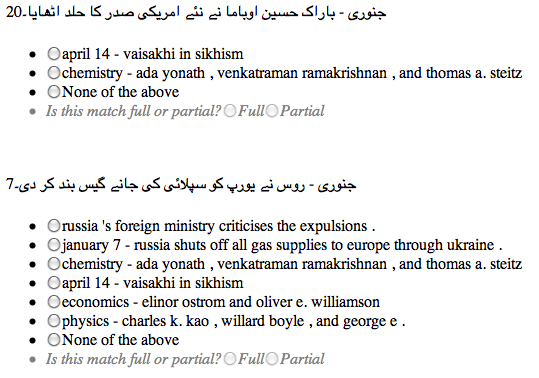
\includegraphics[scale=0.5]{images/turk_hit.png}
\caption{The MTurk annotation interface for finding Urdu-English parallel sentences.}
\label{fig:alignment_hit}
\end{center}
\end{figure}

Our method of pruning potential sentence pairs may leave us with more than ten
candidate English sentences for some Urdu sentences. When this happens, we make
additional questions about these Urdu sentences to ensure all candidate pairs
are accounted for in the annotation. 

In each HIT, we ask the Turkers to annotate up to ten Urdu sentences with their
English counterpart (if any), including two control questions with sentences
taken from the parallel data described in Section \ref{sec:turk_data}. There is
one positive and one negative control in each HIT. We also request that each HIT
be done by three Turkers.

\subsection{Data Collection Results}
\label{sec:turk_results}
In our first large-scale experiment, we took 92 Urdu-English article
pairs, applied our filters as described in Section \ref{sec:turk_data}, and
uploaded our task to MTurk. While there were over 8 million possible sentence
pairs in these articles before pruning, we ended up with $785,000$ sentence
pairs to be annotated at a total cost of $\$726.80$ (this cost includes the duplicate
annotations).

Agreement among the Turkers was high ($\kappa = 0.84$). While the most common
answer was ``None of the above'', there were a substantial number of Urdu
sentences which the Turkers found some English counterpart for. For $21.4\%$ of Urdu
sentences, at least one Turker found one of the English sentences to be
parallel, and in $44.8\%$ of Urdu sentences, at least two Turkers identified a match.

% thesis-only: Using this as a way to get parallel data

\subsection{Evaluation Using Partial Alignments}
\label{sec:partial}
When we evaluate our sentence pair alignment model, we would like to compute the
precision and recall of the proposed sentence alignments. However, since we
prune many possible sentence pairs before asking the Turkers for annotation, we
cannot be sure whether or not some sentence pairs are parallel. In this section,
we will outline a scheme for evaluating sentence alignments using our partially
annotated data.

Our primary intrinsic evalutaion metric is alignment F-measure on sentence
alignments. This metric could also be seen as F-measure on a parallel sentence
pair retrieval task. Let $T$ be the set of true positives (sentence pairs that
are truly parallel), and $P$ be the set of predicted positives (sentence pairs
identified by our model as parallel). Precision, recall, and F-measure are
defined as follows:

\begin{align*}
\mbox{Precison}&=& \frac{|T \cup P|}{|P|}\\
\mbox{Recall}&=& \frac{|T \cup P|}{|T|}\\
\mbox{F-measure}&=& \frac{2 \cdot \mbox{Precision} \cdot
\mbox{Recall}}{\mbox{Precision} + \mbox{Recall}}
\end{align*}

When our document pairs are only partially annotated, we will used modified
definitions of precision, recall, and F-measure. Let $U$ be the set of sentence
pairs which were not annotated as parallel or non-parallel.

\begin{align*}
\mbox{Precison}&=& \frac{|T \cup P|}{|P \setminus U|}\\
\mbox{Recall}&=& \frac{|T \cup P|}{|T|}\\
\mbox{F-measure}&=& \frac{2 \cdot \mbox{Precision} \cdot
\mbox{Recall}}{\mbox{Precision} + \mbox{Recall}}
\end{align*}

Since $T$ and $U$ are disjoint, only the definition of precision needs to
be modified. 

Given the annotations we gathered from MTurk, it is possible to define $U$ in
multiple ways. The most conservative method would be to take $U$ to be all
sentence pairs not presented to the Turkers. However, if we make the assumption
that sentence alignments of the document pairs are $1:1$, then when a Turker
annotates a sentence pair $(S, T)$ as parallel, it follows that all $(S, T')$
pairs with $T' \neq T$ and $(S', T)$ pairs with $S' \neq S$ are not parallel.
Since the alignments we found were mostly $1:1$, we decided to go with this
option.\footnote{There were a small number of alignments which were not $1:1$,
most of which were image captions.} Figure \ref{fig:partial_align} illustrates
this method.

\begin{figure}
\begin{center}
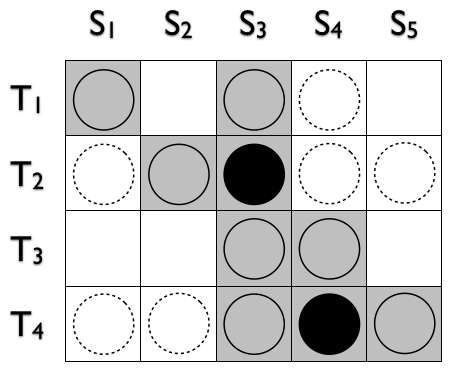
\includegraphics[scale=0.5]{images/partial_alignment.png}
\caption{A partial alignment grid for a comparable document pair. The shaded
cells in the grid represent the sentence pairs which were presented to the
Turkers for annotation. A filled circle indicates the Turker found the sentence
pair to be parallel, and an empty circle means the pair is not parallel. The
dashed circles represent the sentence pairs we infer to be non-parallel by
assuming the sentence alignments are $1:1$.}
\label{fig:partial_align}
\end{center}
\end{figure}

\subsection{Alternate Evaluation Strategies}
% thesis only
Section \ref{sec:partial} describes a method for using Turkers' partial
annotation of a document pair's sentence alignment for intrinsic evaluation of a
sentence alignment model. In this section, we will explore other
strategies for using the Turkers' output for evaluation.

In our MTurk task setup (see Section \ref{sec:design}), we collect redundant
annotations for each HIT. While this was done primarily for quality control, and
it is more convenient to use a single judgement for each sentence pair, we can
perform a more fine-grained analysis by looking at the individual Turkers'
judgements. Also, we gave the option of labeling a parallel sentence pair as a
``partial'' or ``full'' match.

\NoteJS{TODO: For the semi-supervised experiments, we want to treat sentence
pairs that any annotator marked as a match as a true positive. We could also
measure the inter-annotator agreement of our system against the Turkers.}

\section{Experiments}
\label{sec:unsup_experiments}
Our first set of experiments uses a semi-supervised setting. We have both
parallel sentences (labeled data) and comparable document pairs (unlabeled data),
and learn our model's parameters from both of these resources.

Our parallel corpus is taken from the NIST MT09 Urdu-English training set
and the bilingual dictionaries and sentences gathered by
\citet{Post12}.\footnote{This is the same parallel corpus used to create the
sentence pair filters used in collecting the annotated sentence alignments.}
The parallel sentences from this corpus are treated as single sentence document
pairs. Alternatively, the entire training set could be seen as a single document
pair whose sentence alignment lies completely on the diagonal. The model
described in \ref{sec:alignment} does not differentiate between these two ways
of viewing the corpus. In either case, learning from the parallel sentences is
identical to IBM Model 1 training.

The comparable document pairs are a subset of the Wikipedia article pairs that
we annotated using MTurk as described in Section \ref{sec:data}. $60\%$ of this
data was taken as a development set. The remaining $40\%$ of the annotated
document pairs was split into two equal sized test sets.\footnote{This split was
done in order to have training, development, and test sets for supervised
sentence aligment models.}

In the following experiments the setup is as follows: We initialize our
parameters by running five iterations of EM on the parallel sentences from our
labeled data. Then we run several iterations of EM on both the labeled data and
unlabeled data, measuring performance after each iteration.

\subsection{Intrinsic Results}

\subsection{Extrinsic Results}
\NoteJS{This experiments section takes the new strategy where we start with lots
of supervision and then see how well we do as we remove data. Hopefully it will
end with good unsupervised results.}
The ultimate goal of parallel sentence extraction is to improve the quality of
end-to-end machine translation. In this section we will measure MT performance
before and after the extracted parallel sentences are added to the training
data.

\subsubsection{Corpora}
\begin{table*}
\small
\begin{center}
\begin{tabular}{|c|c|c|c|c|c|c|c|}
\hline
French & German & Polish & Italian & Dutch & Portuguese & Spanish & Japanese \\
496K & 488K & 384K & 380K & 357K & 323K & 311K & 252K\\
\hline
Russian & Swedish & Finnish & Chinese & Norwegian & Volap\"{u}k & Catalan & Czech \\
232K & 197K & 146K & 142K & 141K & 106K & 103K & 87K\\
\hline
\end{tabular}
\end{center}
\caption{The sizes of corpora in tokens and sentences for the Spanish-English
condition.}
\label{table:esen_corpora}
\end{table*}

\section{Experiments (Alternate)}
\label{sec:experiments_all}
In this section, we explore the relationship between the amount of initial
parallel data, the quality of the extracted parallel data, and the end-to-end
machine translation quality. We start with Spanish-English as our language pair,
since this is a high resource language pair, and we can always simulate a low
resource setting by restricting the amount of data used.

\subsection{Datasets}
For our initial parallel data, we use the parallel and monolingual corpora
available for the 2010 Machine Translation Workshop's shared task (WMT10). For
the Spanish-English task, the WMT10 data includes Europarl version 5 (we use
version 6 in our experiments\NoteJS{This may change to 7}) \citep{Koehn05}, the United Nations
parallel text, and parallel and monolingual news corpora. Table \ref{table:esen_parallel}
lists the corpora used in detail.

\begin{table*}[ht]
\begin{center}
\begin{tabular}{|rr||r|r|r|}
\hline
      &                & Spanish        & English & English (Monolingual) \\
\hline
\textbf{Europarl} \
      & Sentences     & 1.79M       & 1.79M   & 1.79M   \\
      & Tokens     & 46.8M       & 44.7M   & 44.7M   \\
\hline
\textbf{United Nations} \
      & Sentences     & 6.22M       & 6.22M & 6.22M     \\
      & Tokens     & 191M       & 164M & 164M     \\
\hline
\textbf{News Commentary} \
      & Sentences     & 98.6K       & 98.6K & 126K      \\
      & Tokens     & 2.45M       & 2.10M  & 261M    \\
\hline
\textbf{News} \
      & Sentences     & N/A       & N/A & 48.7M     \\
      & Tokens     & N/A       & N/A & 989M     \\
\hline
\end{tabular}
\end{center}
\caption{Statistics for the initial parallel/monolingual data used in training
baseline MT systems and for extracting new parallel data. The monolingual data
is only used for language modeling, not for extracting parallel sentences.}
\label{table:esen_parallel}
\end{table*}

This data is used both for training the parallel sentence extractor, and as the
initial data in the MT system.

\subsection{Supervised Parallel Sentence Extraction}
In order to extract parallel sentence pairs from Wikipedia, we used a simplified
version of the approach described in \citet{Smith10}.

Using the initial parallel data and a small amount of annotated Spanish-English
Wikipedia articles, we extracted sentence pairs from all of the Spanish-English
Wikipedia articles which were identified as sharing a topic through Wikipedia's
Interwiki link system. This gave us a set of 433 thousand comparable document
pairs. For all pairs of sentences in each document pair, we applied a binary
classifier to determine whether or not the sentence pair was parallel.

Table \ref{table:esen_wiki_parallel} lists the parallel corpora extracted from
Spanish-English article pairs from Wikipedia. ``Wiki@X'' refers to the parallel
sentences extracted with a classification threshold of $X$ (a lower
classification threshold will allow more sentences to be extracted). The
monolingual data was taken from the English side of all Spanish-English document
pairs, making it consistent across conditions.

\begin{table*}[ht]
\begin{center}
\begin{tabular}{|rr||r|r|r|}
\hline
      &                & Spanish        & English & English (Monolingual) \\
\hline
\textbf{Wiki@0.75} \
      & Sentences     &   ---     & --- & 14.8M     \\
      & Tokens     &  ---      & --- & 286M    \\
\hline
\textbf{Wiki@0.5} \
      & Sentences     & 1.60M       & 1.60M & 14.8M     \\
      & Tokens     & 44.8M       & 51.0M & 286M     \\
\hline
\textbf{Wiki@0.25} \
      & Sentences     &   ---     & --- & 14.8M     \\
      & Tokens     &  ---      & --- & 286M    \\
\hline
\end{tabular}
\end{center}
\caption{Statistics for parallel corpora extracted from Wikipedia.}
\label{table:esen_wiki_parallel}
\end{table*}

\subsection{Results}
We report end-to-end MT results using the initial parallel data and the
extracted parallel data from Wikipedia. For our baseline MT system we used the
phrase-based model included in the Moses toolkit \citet{Koehn07} with all
options set to the default. % TODO: Cite Edinburgh submission

We used two test sets to evaluate the end-to-end MT performance: the test set
from WMT10 which was taken from the news domain, and a set of parallel sentences
from Wikipedia gathered by \citep{Smith10}.

\begin{table*}[ht]
\begin{center}
\begin{tabular}{|r||r|r|}
\hline
      & WMT10        & Wikipedia \\
\hline
\textbf{Europarl Only} \
      & 24.75       & ---    \\
\textbf{+Wiki LM} \
      & 26.91       & ---    \\
\textbf{+Wiki Parallel (@0.75)} \
      & ---       & ---    \\
\textbf{+Wiki Parallel (@0.5)} \
      & 27.41       & ---    \\
\textbf{+Wiki Parallel (@0.25)} \
      & ---       & ---    \\
\hline
\textbf{All Initial Corpora} \
      & 28.51       & ---    \\
\textbf{+Wiki LM} \
      & 28.55       & ---    \\
\textbf{+Wiki Parallel (@0.75)} \
      & ---       & ---    \\
\textbf{+Wiki Parallel (@0.5)} \
      & 29.23       & ---    \\
\textbf{+Wiki Parallel (@0.25)} \
      & ---       & ---    \\
\hline
\end{tabular}
\end{center}
\caption{BLEU scores for systems trained on different sets of parallel and
monolingual data before and after adding data from Wikipedia.}
\label{table:esen_bleu}
\end{table*}

\section{Conclusions}
